\section{Computing Gradients of Tensor Networks}\label{chapter:gradients}
Optimizing tensor networks in a general setting is a significant challenge in many research areas. Although many optimization techniques have been developed for matrices, extending these methods to tensor networks can remain challenging~\citep{liao2019differentiable}. This complexity stems from the high computational cost of tensor contractions and the lack of efficient optimization algorithms for higher-dimensional cases. Additionally, manually computing gradients using the chain rule can seem daunting beyond simple tensor network structures. In this chapter, we introduce an elegant and intuitive approach for deriving higher-order derivatives using the graphical notation of a tensor network. This approach illustrates that derivatives of tensor network functions often inherit the low-rank structure of the initial tensor network.

In the next section, we first define the classical concepts of gradient and Jacobian for functions that take vectors as input. We then extend these concepts to functions that take tensors as inputs and produce tensors as outputs.
\subsection{Jacobians}
We first recall the classical notions of gradient and Jacobian of functions defined over $\mathbb{R}^n$.

\begin{definition}
  For $f:\RR^n\to\RR$ and $g:\RR^n\to\RR^p$. The gradient of $f$ and the Jacobian of $g$ at $\theta\in\mathbb{R}^n$ are defined by
    $$\nabla_\theta f = \left[\frac{\partial f(\theta)}
{\partial\theta_1},\frac{\partial f(\theta)}{\partial\theta_2},\dots,\frac{\partial f(\theta)} 
    {\partial\theta_n}\right]^\ts
        =
    \begin{tikzpicture}[baseline=\baseline]
    \tikzset{tensor/.style = {minimum size = 0.5cm,shape = circle,thick,draw=black,inner sep = 0pt}, edge/.style   = {thick,line width=.4mm}}
    \def\y{0}
     \def\x{0}
    \node[tensor,fill=blue!40!red!60!white] (a1) at (\x,\y){};
    \draw[edge](a1) -- (\x+0.75,\y)node [midway, above]{\edgelabel{$n$}};
    \end{tikzpicture} \in\mathbb{R}^n,$$
    and 
    $$\frac{\partial g(\theta)}{\partial\theta} = \left(\frac{\partial g(\theta)_i}{\partial\theta_j}\right)_{i=1,\cdots,p\atop j=1,\cdots, n}
    =
    \begin{tikzpicture}[baseline=\baseline]
    \tikzset{tensor/.style = {minimum size = 0.5cm,shape = circle,thick,draw=black,inner sep = 0pt}, edge/.style   = {thick,line width=.4mm}}
    \def\y{0}
     \def\x{0}
    \node[tensor,fill=blue!20!red!50!white] (A) at (\x,\y){};
    \draw[edge](A) -- (\x+0.75,\y)node [midway, above]{\scalebox{0.7}{\dimcolor{$n$}}};
    \draw[edge](A) -- (\x-0.75,\y)node [midway, above]{\scalebox{0.7}{\dimcolor{$p$}}};
    \end{tikzpicture}\in\mathbb{R}^{p\times n}.$$  
\end{definition}
We can naturally extend the notion of Jacobian to functions that take tensors as input and output tensors~(of arbitrary orders).

\begin{definition}
 Let $f:\RR^{n_1\times\dots\times n_N}\to\RR^{m_1\times\dots\times m_M}$,. The \emph{Jacobian tensor} of $f$ at $\theta\in\RR^{n_1\times\dots\times n_N}$ is the tensor $\frac{\partial f}{\partial\theta}\in\RR^{m_1\times\dots\times m_M\times n_1\times\dots\times n_N}$
 defined by
\begin{align*}
   \frac{\partial f(\theta)}{\partial\theta} 
   &= 
   \left(\frac{\partial f(\theta)_{i_1,\dots,i_M}}{\partial\theta_{j_1,\dots,j_N}}\right)_{i_1\in[m_1],\cdots,i_M\in[m_M]\atop j_1\in[n_1],\cdots,j_N
\in[n_N]}\\
&=
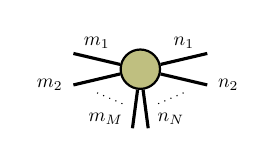
\begin{tikzpicture}[baseline=-0.5ex]
    \tikzset{tensor/.style = {minimum size = 0.5cm,shape = circle,thick,draw=black,inner sep = 0pt}, edge/.style = {thick,line width=.4mm},every loop/.style={}}
    \def\x{6}
    \node[tensor,fill=green!50!red!50!white] (T) at (\x,0) {};
    \draw[edge] (T) -- (\x-0.85,0.2)node [midway, above]{\scalebox{0.7}{\dimcolor{$m_1$}}};
    \draw[edge] (T) -- (\x-0.85,-0.2)node [left]{\scalebox{0.7}{\dimcolor{$m_2$}}};
    \draw[edge] (T) -- (\x-0.1,-0.75)node [near end, left]{\scalebox{0.7}{\dimcolor{$m_M$}}};
    \draw[dotted] (\x-0.55,-0.3) -- (\x-0.2,-0.45);
    \draw[edge] (T) -- (\x+0.85,0.2)node [midway, above]{\scalebox{0.7}{\dimcolor{$n_1$}}};
    \draw[edge] (T) -- (\x+0.85,-0.2)node [right]{\scalebox{0.7}{\dimcolor{$n_2$}}};
    \draw[edge] (T) -- (\x+0.1,-0.75)node [near end, right]{\scalebox{0.7}{\dimcolor{$n_N$}}};
    \draw[dotted] (\x+0.55,-0.3) -- (\x+0.2,-0.45);
    \end{tikzpicture}\in\RR^{m_1\times\cdots\times m_M\times n_1\times\cdots\times n_N}. 
\end{align*}
\end{definition}




The following theorem demonstrates that first-order derivatives of tensor networks with respect to a core tensor can be easily computed using tensor networks.

\begin{theorem}\label{thm:gradients}
    Let $\Tt$ be a tensor given as a tensor network, where $\Gt$ is a core tensor \emph{appearing only once} in the tensor network. Then $\frac{\partial \Tt}{\partial \Gt}$ is obtained by removing $\Gt$ from the tensor network of $\Tt$. 
\end{theorem}
The following examples illustrate how Theorem~\ref{thm:gradients} can be applied to tensor networks.
\paragraph{Examples}
Let 
$\begin{tikzpicture}[baseline=\baseline]
    \tikzset{tensor/.style = {minimum size = 0.5cm,shape = circle,thick,draw=black,inner sep = 0pt}, edge/.style = {thick,line width=.4mm},every loop/.style={}}
    \def\x{0}
    \def\y{0}
     \node[tensor,fill=green!50!red!50!white] (B) at (\x+1,\y) {$\Xt$};
    \draw[edge] (B) -- (\x+0.25,0) node [midway,above] {\scalebox{0.7}{\dimcolor{$d_1$}}};
    \draw[edge] (B) -- (\x+1.85,\y) node [midway,above] {\scalebox{0.7}{\dimcolor{$d_3$}}};
    \draw[edge] (B) -- (\x+1,\y-0.85) node [midway,left] {\scalebox{0.7}{\dimcolor{$d_2$}}};
\end{tikzpicture}
=
\begin{tikzpicture}[baseline=\baseline]
    \tikzset{tensor/.style = {minimum size = 0.5cm,shape = circle,thick,draw=black,inner sep = 0pt}, edge/.style = {thick,line width=.4mm},every loop/.style={}}
    \def\x{0}
    \def\y{0}
    \node[tensor,fill=red!30!white] (A) at (\x+2,\y) {$\Gt_1$};
    \node[tensor,fill=red!50!white] (B) at (\x+3.2,\y) {$\Gt_2$};
    \node[tensor,fill=blue!30!white] (C) at (\x+2.6,\y-0.7) {$\Gt_3$};
    \node[tensor,fill=blue!50!white] (D) at (\x+4.3,\y) {$\Gt_4$};
    \draw[edge] (A) -- (B) node [midway,above] {\scalebox{0.7}{\dimcolor{$R_1$}}};
    \draw[edge] (A) -- (C);
    \node[draw=none] () at (\x+2,\y-0.5) {\scalebox{0.7}{\dimcolor{$R_2$}}};
    \draw[edge] (B) -- (C);
    \node[draw=none] () at (\x+3.2,\y-0.5) {\scalebox{0.7}{\dimcolor{$R_3$}}};
    \draw[edge] (B) -- (D) node [midway,above] {\scalebox{0.7}{\dimcolor{$R_4$}}};
    \draw[edge] (A) -- (\x+2,\y+0.7) node [midway,left] {\scalebox{0.7}{\dimcolor{$d_1$}}};
    \draw[edge] (D) -- (\x+4.3,\y+0.7) node [midway,right] {\scalebox{0.7}{\dimcolor{$d_3$}}};
    \draw[edge] (C) -- (\x+2.6,\y-1.5) node [midway,left] {\scalebox{0.7}{\dimcolor{$d_2$}}};
\end{tikzpicture}
$ be a tensor network. Observe that we can think of $\Xt$ as a function of any of the core tensors of its tensor network representation. We can thus naturally ask what the Jacobian of $\Xt$ is with respect to, e.g., $\Gt_2$ or $\Gt_4$.
The previous theorem gives us an easy way to compute these derivatives:
\begin{itemize}
\item According to Theorem~\ref{thm:gradients}, to find the gradient of $\Xt$ with respect to $\Gt_2$, we need to remove the core $\Gt_2$ from the tensor network, i.e.,
$$
\frac{\partial}{\partial\Gt_2}\left(\begin{tikzpicture}[baseline=\baseline]
    \tikzset{tensor/.style = {minimum size = 0.5cm,shape = circle,thick,draw=black,inner sep = 0pt}, edge/.style = {thick,line width=.4mm},every loop/.style={}}
    \def\y{0}
    \def\x{0}
    \node[tensor,fill=red!30!white] (A) at (\x+2,\y) {$\Gt_1$};
    \node[tensor,fill=red!50!white] (B) at (\x+3.2,\y) {$\Gt_2$};
    \node[tensor,fill=blue!30!white] (C) at (\x+2.6,\y-0.7) {$\Gt_3$};
    \node[tensor,fill=blue!50!white] (D) at (\x+4.3,\y) {$\Gt_4$};
    \draw[edge] (A) -- (B) node [midway,above] {\scalebox{0.7}{\dimcolor{$R_1$}}};
    \draw[edge] (A) -- (C);
    \node[draw=none] () at (\x+2,\y-0.5) {\scalebox{0.7}{\dimcolor{$R_2$}}};
    \draw[edge] (B) -- (C);
    \node[draw=none] () at (\x+3.2,\y-0.5) {\scalebox{0.7}{\dimcolor{$R_3$}}};
    \draw[edge] (B) -- (D) node [midway,above] {\scalebox{0.7}{\dimcolor{$R_4$}}};
    \draw[edge] (A) -- (\x+2,\y+0.7) node [midway,left] {\scalebox{0.7}{\dimcolor{$d_1$}}};
    \draw[edge] (D) -- (\x+4.3,\y+0.7) node [midway,right] {\scalebox{0.7}{\dimcolor{$d_3$}}};
    \draw[edge] (C) -- (\x+2.6,\y-1.5) node [midway,left] {\scalebox{0.7}{\dimcolor{$d_2$}}};
    \end{tikzpicture}\right)
=
    \begin{tikzpicture}[baseline=\baseline]
    \tikzset{tensor/.style = {minimum size = 0.5cm,shape = circle,thick,draw=black,inner sep = 0pt}, edge/.style = {thick,line width=.4mm},every loop/.style={}}
    \def\y{-0.5}
    \def\x{0}
    \node[tensor,fill=red!30!white] (A) at (\x,\y+1) {$\Gt_1$};
    \node[tensor,fill=blue!30!white] (C) at (\x+0.6,\y+0.2) {$\Gt_3$};
    \node[tensor,fill=blue!50!white] (D) at (\x+2,\y+0.5) {$\Gt_4$};
    \draw[edge] (A) -- (C);
    \draw[edge] (A) -- (\x,\y+1.7) node [midway,left] {\scalebox{0.7}{\dimcolor{$d_1$}}};
    \draw[edge] (A) -- (\x+0.7,\y+1) node [midway,above] 
{\scalebox{0.7}{\dimcolor{$R_1$}}};
    \draw[edge] (D) -- (\x+3,\y+0.5) node [midway,above] {\scalebox{0.7}{\dimcolor{$R_4$}}};
    \draw[edge] (C) -- (\x+0.6,\y-0.7) node [midway,left] {\scalebox{0.7}{\dimcolor{$d_2$}}};
    \draw[edge] (C) -- (\x+1.3,\y+0.2) node [midway,above] {\scalebox{0.7}{\dimcolor{$R_3$}}};
    \draw[edge] (D) -- (\x+2,\y+1.3) node [midway,left] {\scalebox{0.7}{\dimcolor{$d_3$}}};
    \node[draw=none] () at (\x,\y+0.4) {\scalebox{0.7}{\dimcolor{$R_2$}}};
\end{tikzpicture}.
$$ 
To understand why this procedure works, we can view the tensor decomposition of $\Xt$ as a matrix-vector product:
$$
\Mb\vb 
=
\begin{tikzpicture}[baseline=\baseline]
    \tikzset{tensor/.style = {minimum size = 0.5cm,shape = circle,thick,draw=black,inner sep = 0pt}, edge/.style = {thick,line width=.4mm},every loop/.style={}}
    \def\y{1}
    \def\x{0}
     \node[tensor,fill=red!30!white](G_1) at (\x,\y) {$\Gt_1$};
    \node[tensor,fill=blue!30!white] (G_3) at (\x,\y-1) {$\Gt_3$};
     \node[tensor,fill=red!50!white](G_2) at (\x+2,\y-1) {$\Gt_2$};
    \node[tensor,fill=blue!50!white] (G_4) at (\x,\y-2) {$\Gt_4$};
    \node[tensor,fill=red!50!white] (G_2) at (\x+2,\y-1) {$\Gt_2$};
    \draw[edge](G_1) -- (\x-1,\y) -- (\x-1,\y-0.85) -- (\x-1.75,\y-0.85);
    \draw[edge](G_3)-- (\x-1.75,\y-1)node [left] {\scalebox{0.7}{\dimcolor{$d_1d_2d_3$}}};
    \draw[edge](G_2)--(G_1)node [midway,above] {\scalebox{0.7}{\dimcolor{$R_1$}}};
    \draw[edge](G_2)--(G_3)node [midway,above] {\scalebox{0.7}{\dimcolor{$R_3$}}};
    \draw[edge](G_1)--(G_3)node [midway,left] {\scalebox{0.7}{\dimcolor{$R_2$}}};
    \draw[edge](G_2)--(G_4)node [midway,above] {\scalebox{0.7}{\dimcolor{$R_4$}}};
    \draw[edge] (G_4) -- (\x-1,\y-2) -- (\x-1,\y-1.15) -- (\x-1.75,\y-1.15);
    \draw[dotted] (\x+0.45,\y+0.65) -- (\x+0.45,\y-2.35);
\end{tikzpicture},
$$
where $\vb = \vectorize(\Gt_2) $ and $\Mb$ is the matrix obtained by matricization of the remaining part of the tensor network. 
Using the classical identity for the Jacobian of a linear map, the expected result is obtained:
$$\frac{\partial\Mb\vb}{\partial\vb} = \Mb = 
\begin{tikzpicture}[baseline=\baseline]
    \tikzset{tensor/.style = {minimum size = 0.5cm,shape = circle,thick,draw=black,inner sep = 0pt}, edge/.style = {thick,line width=.4mm},every loop/.style={}}
    \def\y{1}
    \def\x{0}
     \node[tensor,fill=red!30!white](G_1) at (\x,\y) {$\Gt_1$};
    \node[tensor,fill=blue!30!white] (G_3) at (\x,\y-1) {$\Gt_3$};
    \node[tensor,fill=blue!50!white] (G_4) at (\x,\y-2) {$\Gt_4$};
    \draw[edge](G_1) -- (\x-0.85,\y) -- (\x-0.85,\y-0.9) -- (\x-1.5,\y-0.9);
    \draw[edge](G_3)-- (\x-1.5,\y-1)node [left] {\scalebox{0.7}{\dimcolor{$d_1d_2d_3$}}};
    \draw[edge](G_1)-- (\x+0.85,\y) -- (\x+0.85,\y-0.9) -- (\x+1.5,\y-0.9);
    \draw[edge](G_3) -- (\x+1.5,\y-1) node [right] {\scalebox{0.7}{\dimcolor{$R_1R_3R_4$}}};
    \draw[edge](G_1)--(G_3)node [midway,left] {\scalebox{0.7}{\dimcolor{$R_2$}}};
    \draw[edge] (G_4) -- (\x+0.85,\y-2) -- (\x+0.85,\y-1.1) -- (\x+1.5,\y-1.1);
    \draw[edge] (G_4) -- (\x-0.85,\y-2) -- (\x-0.85,\y-1.1) -- (\x-1.5,\y-1.1);
\end{tikzpicture}\in\RR^{d_1d_2d_3\times R_1R_3R_4}.
$$
\item According to Theorem~\ref{thm:gradients} to find the gradient of $\Xt$ with respect to $\Gt_4$, we need to remove the core $\Gt_4$ from the corresponding tensor network. i.e., 
$$
    \frac{\partial}{\partial\Gt_4}\left(\begin{tikzpicture}[baseline=\baseline]
    \tikzset{tensor/.style = {minimum size = 0.5cm,shape = circle,thick,draw=black,inner sep = 0pt}, edge/.style = {thick,line width=.4mm},every loop/.style={}}
    \def\x{0}
    \def\y{0}
    \node[tensor,fill=red!30!white] (A) at (\x+2,\y) {$\Gt_1$};
    \node[tensor,fill=red!50!white] (B) at (\x+3.2,\y) {$\Gt_2$};
    \node[tensor,fill=blue!30!white] (C) at (\x+2.6,\y-0.7) {$\Gt_3$};
    \node[tensor,fill=blue!50!white] (D) at (\x+4.3,\y) {$\Gt_4$};
    \draw[edge] (A) -- (B) node [midway,above] {\scalebox{0.7}{\dimcolor{$R_1$}}};
    \draw[edge] (A) -- (C);
    \node[draw=none] () at (\x+2,\y-0.5) {\scalebox{0.7}{\dimcolor{$R_2$}}};
    \draw[edge] (B) -- (C);
    \node[draw=none] () at (\x+3.2,\y-0.5) {\scalebox{0.7}{\dimcolor{$R_3$}}};
    \draw[edge] (B) -- (D) node [midway,above] {\scalebox{0.7}{\dimcolor{$R_4$}}};
    \draw[edge] (A) -- (\x+2,\y+0.7) node [midway,left] {\scalebox{0.7}{\dimcolor{$d_1$}}};
    \draw[edge] (D) -- (\x+4.3,\y+0.7) node [midway,right] {\scalebox{0.7}{\dimcolor{$d_3$}}};
    \draw[edge] (C) -- (\x+2.6,\y-1.5) node [midway,left] {\scalebox{0.7}{\dimcolor{$d_2$}}};
    \end{tikzpicture}\right)
=
    \begin{tikzpicture}[baseline=\baseline]
    \tikzset{tensor/.style = {minimum size = 0.5cm,shape = circle,thick,draw=black,inner sep = 0pt}, edge/.style = {thick,line width=.4mm},every loop/.style={}}
    \def\y{-0.5}
    \def\x{0}
    \node[tensor,fill=red!30!white] (A) at (\x+2,\y+1) {$\Gt_1$};
    \node[tensor,fill=red!50!white] (B) at (\x+3.2,\y+1) {$\Gt_2$};
    \node[tensor,fill=blue!30!white] (C) at (\x+2.6,\y) {$\Gt_3$};
    \draw[edge] (A) -- (B) node [midway,above] {\scalebox{0.7}{\dimcolor{$R_1$}}};
    \draw[edge] (A) -- (C);
    \node[draw=none] () at (\x+2,\y+0.5) {\scalebox{0.7}{\dimcolor{$R_2$}}};
    \draw[edge] (B) -- (C);
    \node[draw=none] () at (\x+3.2,\y+0.5) {\scalebox{0.7}{\dimcolor{$R_3$}}};
    \draw[edge] (B) -- (\x+4,\y+1) node [midway,above] {\scalebox{0.7}{\dimcolor{$R_4$}}};
    \draw[edge] (A) -- (\x+2,\y+1.7) node [midway,left] {\scalebox{0.7}{\dimcolor{$d_1$}}};
    \draw[edge] (C) -- (\x+2.6,\y-0.7) node [midway,left] {\scalebox{0.7}{\dimcolor{$d_2$}}};
    \draw[edge] (\x+4.5,\y+1) -- (\x+4.5,\y+1.65) node [midway,right] {\scalebox{0.7}{\dimcolor{$d_3$}}};
    \end{tikzpicture}.
$$
Observe that the dangling leg of $\Gt_4$ remains in the Jacobian tensor! To understand why this is the case, we can again view the tensor decomposition of $\Xt$ as a matrix-vector product $\Mb\vb$, such that 
$$
\Mb\vb = \begin{tikzpicture}[baseline=\baseline]
    \tikzset{tensor/.style = {minimum size = 0.5cm,shape = circle,thick,draw=black,inner sep = 0pt}, edge/.style = {thick,line width=.4mm},every loop/.style={}}
    \def\y{0.7}
    \def\x{0}
     \node[tensor,fill=red!30!white](G_1) at (\x,\y) {$\Gt_1$};
     \node[tensor,fill=red!50!white](G_2) at (\x+1,\y) {$\Gt_2$};
    \node[tensor,fill=blue!30!white] (G_3) at (\x+0.5,\y-1) {$\Gt_3$};
    \node[tensor,fill=blue!50!white] (G_4) at (\x+2.25,\y-1.5) {$\Gt_4$};
    \draw[edge](G_2)--(G_3);
    \draw[edge](G_1)--(G_2)node [midway,above] {\scalebox{0.7}{\dimcolor{$R_1$}}};
    \draw[edge](G_1)--(G_3);
    \draw[edge](G_2)--(G_4)node [midway,above=0.05cm] {\scalebox{0.7}{\dimcolor{$R_4$}}};
    \draw[edge](G_1) -- (\x,\y-1.35) -- (\x+0.35,\y-1.35) -- (\x+0.35,\y-2);
    \draw[edge](G_3)--(\x+0.5,\y-2)node [below] {\scalebox{0.7}{\dimcolor{$d_1d_2d_3$}}};
    \draw[edge](G_4) -- (\x+0.75,\y-1.5) -- (\x+0.75,\y-2);
    \draw[dotted] (\x+2.25,\y-0.75) -- (\x+1,\y-2);
\end{tikzpicture},
$$
where now $\vb  =\vectorize(\Gt_4)$.
Taking derivative of this tensor network with respect to $\vb = \vectorize(\Gb_4)$~gives us the expected result:  $$\frac{\partial\Mb\vb}{\partial\vb} = \Mb
=
\begin{tikzpicture}[baseline=\baseline]
\tikzset{tensor/.style = {minimum size = 0.5cm,shape = circle,thick,draw=black,inner sep = 0pt}, edge/.style = {thick,line width=.4mm},every loop/.style={}}
    \def\y{1}
    \def\x{0}
     \node[tensor,fill=red!30!white](G_1) at (\x,\y) {$\Gt_1$};
     \node[tensor,fill=red!50!white](G_2) at (\x+1,\y) {$\Gt_2$};
    \node[tensor,fill=blue!30!white] (G_3) at (\x+0.5,\y-1) {$\Gt_3$};
    \draw[edge](G_2)--(G_3);
    \draw[edge](G_1)--(G_2)node [midway,above] {\scalebox{0.7}{\dimcolor{$R_1$}}};
    \draw[edge](G_1)--(G_3);
    \draw[edge](G_1) -- (\x,\y-1.35) -- (\x+0.35,\y-1.35) -- (\x+0.35,\y-2);
    \draw[edge](G_3)--(\x+0.5,\y-2)node [below] {\scalebox{0.7}{\dimcolor{$d_1d_2d_3$}}};
     \draw[edge](G_2) -- (\x+1.85,\y)node [midway, above] {\scalebox{0.7}{\dimcolor{$R_4$}}};
    \draw[edge](\x+1.85,\y-1.5) -- (\x+0.75,\y-1.5) -- (\x+0.75,\y-2);
\end{tikzpicture}\in\RR^{d_1d_2d_3\times R_4}.$$
Note that taking the derivative with respect to a tensor removes only the corresponding node from the network, but leaves its connecting edges (legs) intact.
\end{itemize}
We now illustrate how Theorem~\ref{thm:gradients} can be used to effortlessly recover classical derivatives and gradient computations. 
\paragraph{Re-deriving Classical Identities with Tensor Networks}
\begin{enumerate}
\item 
    $\frac{\partial\langle\ub,\vb\rangle}{\partial \ub}
=
    \frac{\partial\left(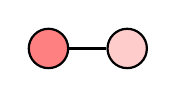
\begin{tikzpicture}[baseline=-0.1ex]
    \tikzset{tensor/.style = {minimum size = 0.5cm,shape = circle,thick,draw=black,inner sep = 0pt}, edge/.style = {thick,line width=.4mm},every loop/.style={}}
    \def\x{0}
    \def\y{0}
    \node[tensor,fill=red!50!white] (u) at (\x+1,\y) {$\ub$};
    \node[tensor,fill=red!20!white] (v) at (\x+2,\y) {$\vb$};
    \draw[edge] (u) -- (v);
    \end{tikzpicture}\right)}{\partial\left(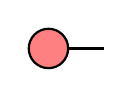
\begin{tikzpicture}[baseline=-0.1ex]
    \tikzset{tensor/.style = {minimum size = 0.5cm,shape = circle,thick,draw=black,inner sep = 0pt}, edge/.style = {thick,line width=.4mm},every loop/.style={}}
    \def\x{0}
    \def\y{0}
    \node[tensor,fill=red!50!white] (u) at (\x+1,\y) {$\ub$};
    \draw[edge] (u) -- (\x+1.7,\y);
    \end{tikzpicture}\right)}
=
    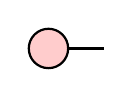
\begin{tikzpicture}[baseline=-0.1ex]
    \tikzset{tensor/.style = {minimum size = 0.5cm,shape = circle,thick,draw=black,inner sep = 0pt}, edge/.style = {thick,line width=.4mm},every loop/.style={}}
    \def\x{6}
    \def\y{0}
    \node[tensor,fill=red!20!white] (v) at (\x+2,\y) {$\vb$};
    \draw[edge] (v) -- (\x+2.7,\y);
    \end{tikzpicture}
    =
    \vb
    $
